\section{实验原理}
\subsection{物理实验原理}


 \begin{figure}[H]
    \centering
    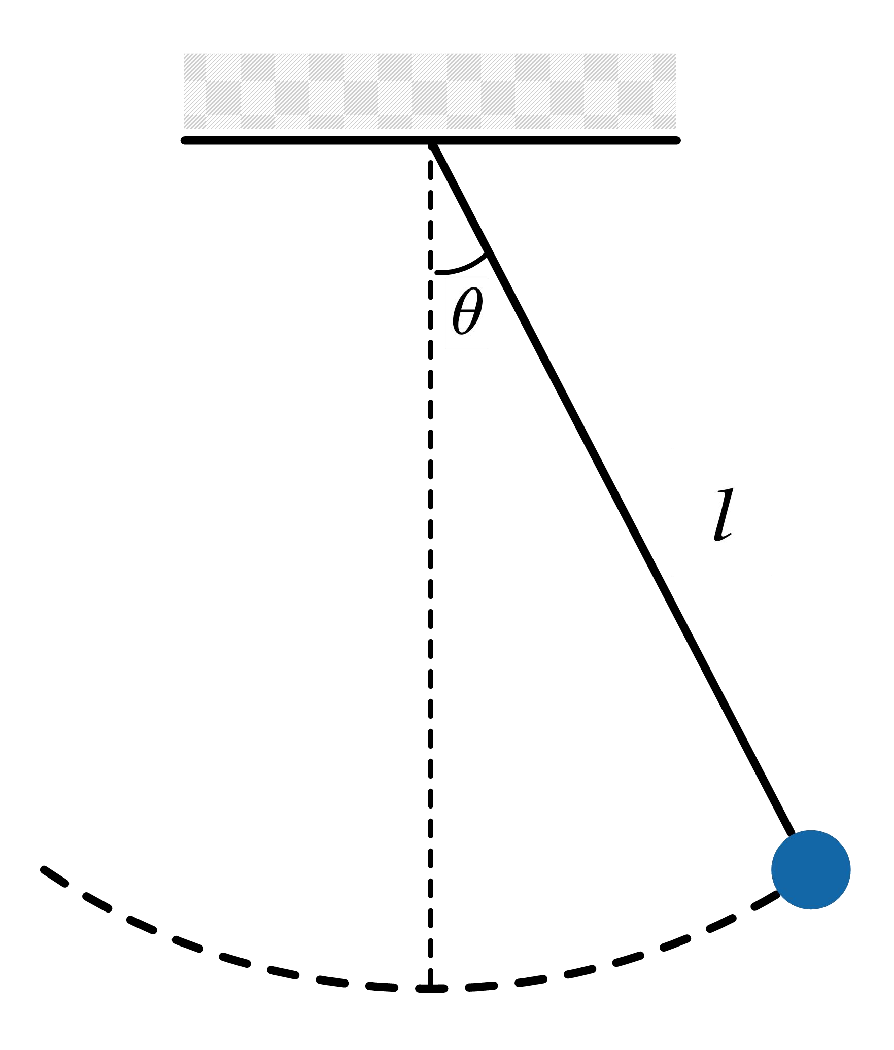
\includegraphics[width=0.2\textwidth]{figures/单摆}
    \caption{单摆模型示例图}
    \label{单摆}
 \end{figure}

 单摆是由一根无弹性的轻质细线和悬在此线一端的摆球组成。若将悬挂的摆球自平衡位置拉至一边,然后释放,摆球则在平衡位置左右作周期性的往返摆动,如图\ref{单摆}所示。

根据受力分析,单摆沿切线方向的回复力为:
\begin{equation}
f = -mg \sin \theta
\end{equation}
式中负号表示回复力方向与角位移 $\theta$ 相反。

根据牛顿第二定律,质点的加速度为 $a = \frac{f}{m}$,代入上式可得:
\begin{equation}
a = -g \sin \theta
\end{equation}

在单摆运动中,质点沿弧线运动,其角加速度可以表示为 $\alpha = \frac{d^2\theta}{dt^2}$,其中 $\alpha=\frac{a}{l}$ ,将其代入上式,得到:

\begin{equation}
\frac{d^2\theta}{dt^2} + \frac{g}{l} \sin \theta = 0
\end{equation}

令 $\omega^2 = \frac{g}{l}$,则方程可简化为:
\begin{equation}
\frac{d^2\theta}{dt^2} + \omega^2 \sin \theta = 0
\end{equation}

这便是单摆运动的微分方程,当$\theta$较小时(小于5°),$\sin \theta \approx \theta$,则方程可简化为:
\begin{equation}
\frac{d^2\theta}{dt^2} + \omega^2 \theta = 0
\end{equation}

\begin{TertiaryBox}[重力加速度测量原理]
根据微分方程理论,该方程的一般解为:
\begin{equation}
    \theta(t) = \theta_0 \cos(\omega t + \varphi_0)
\end{equation}

其中$\theta_0$为初始振幅,$\varphi_0$为初相位,$\omega$为角频率。将此解代入原微分方程式得:

\begin{equation}
  \omega = \sqrt{\frac{g}{l}}
\end{equation}

由振动周期$T$与角频率$\omega$的关系:$T = \frac{2\pi}{\omega}$,代入得:
\begin{equation}
T = \frac{2\pi}{\sqrt{\frac{g}{l}}} = 2\pi\sqrt{\frac{l}{g}}
\end{equation}
所以振动周期为:
\begin{equation}
T = 2\pi\sqrt{\frac{l}{g}}
\end{equation}
\end{TertiaryBox}

这表明单摆的振动周期只与摆长$l$和重力加速度$g$有关,与角振幅$\theta_0$无关,在实际测量中只需要测量出摆长$l$和周期$T$,就可以计算出重力加速度$g$。



\begin{TertiaryBox}[阻尼系数测量原理]
考虑空气阻尼的影响,运动方程修正为:
\begin{equation}
\frac{d^2\theta}{dt^2} + \frac{\beta}{m} \frac{d\theta}{dt} + \omega^2 \theta = 0
\end{equation}

其中 $\beta$ 为单摆系统的阻尼系数(单位:N$\cdot$s/m),$m$为摆球质量,其解为:
\begin{equation}
\theta(t) = \theta_0 e^{-\frac{\beta}{m} t} \cos(\omega t + \varphi_0)
\end{equation}
该解表示阻尼振动,在时间推移后角振幅逐渐衰减。
若测得初始角振幅 $\theta_0$ 和 $n$ 个周期后角振幅 $\theta_n$,则有:
\begin{equation}
\frac{\theta_0}{\theta_n} = \frac{\theta_0}{\theta_0 e^{-\frac{\beta}{m} nT}} = e^{\frac{\beta}{m} nT}
\end{equation}
取对数得阻尼系数:
\begin{equation}
\beta = \frac{m}{nT} \ln\left(\frac{\theta_0}{\theta_n}\right)
\end{equation}
\end{TertiaryBox}

在实际测量中,由于角振幅$\theta$难测量,可将其转化为测量摆球的水平振幅$A$,
根据$A = l\sin \theta,sin \theta \approx \theta$,可得$A = l\theta$,故:
$\beta = \frac{m}{nT} \ln\left(\frac{A_0}{A_n}\right)$,该式中$\frac{A_0}{A_n}$为振幅衰减比,像素振幅衰减比与实际振幅衰减比相同,故不需要将像素长度转换为实际长度。

以上结论均是在小角度近似下得出的,当$\theta$较大时,需要考虑非线性项的影响,摆球的周期$T$为与$\theta$有关,表达式\textsuperscript{\cite{DXWL200705004}}为:
\begin{equation}
T = 4 \sqrt{\frac{l}{g}} \int_{0}^{\frac{\pi}{2}} \frac{1}{\sqrt{1 - \sin^2 \frac{\alpha}{2} \sin^2 \varphi}} \, d\varphi
  = 2\pi\sqrt{\frac{l}{g}} \left( 1 + \sum_{n=1}^{\infty} \left( \frac{(2n-1)!!}{(2n)!!} \right)^2 \sin^{2n} \frac{\alpha}{2} \right)
\end{equation}


\subsection{AI技术原理}

YOLO 是目前为止最先进的目标检测方案之一\textsuperscript{\cite{7780460}},它能够在一幅图面中同时检测并分类出对象。

\subsubsection{YOLO 的神经网络结构}

YOLOv1\textsuperscript{\cite{DBLP:journals/corr/RedmonDGF15}}(2015 年)首次提出将图像划分为 S×S 网格(grid cell),每个网格预测B 个边界框(每个框包含位置坐标和置信度)和 C 个类别概率,最终输出张量维度为S×S×(B×5+C)。其网络结构分为两部分:

特征提取层:
采用 24 层卷积层(借鉴 GoogleNet 的 Inception 模块改进),通过 1×1 和 3×3 卷积组合提取多尺度特征,并交替使用最大池化层压缩特征图尺寸。

预测层:
包含 2 个全连接层,将特征图展平后直接回归边界框坐标和类别概率。输出层使用线性激活函数处理坐标,Sigmoid 函数处理置信度和类别概率。
 \begin{figure}[ht]
    \centering
    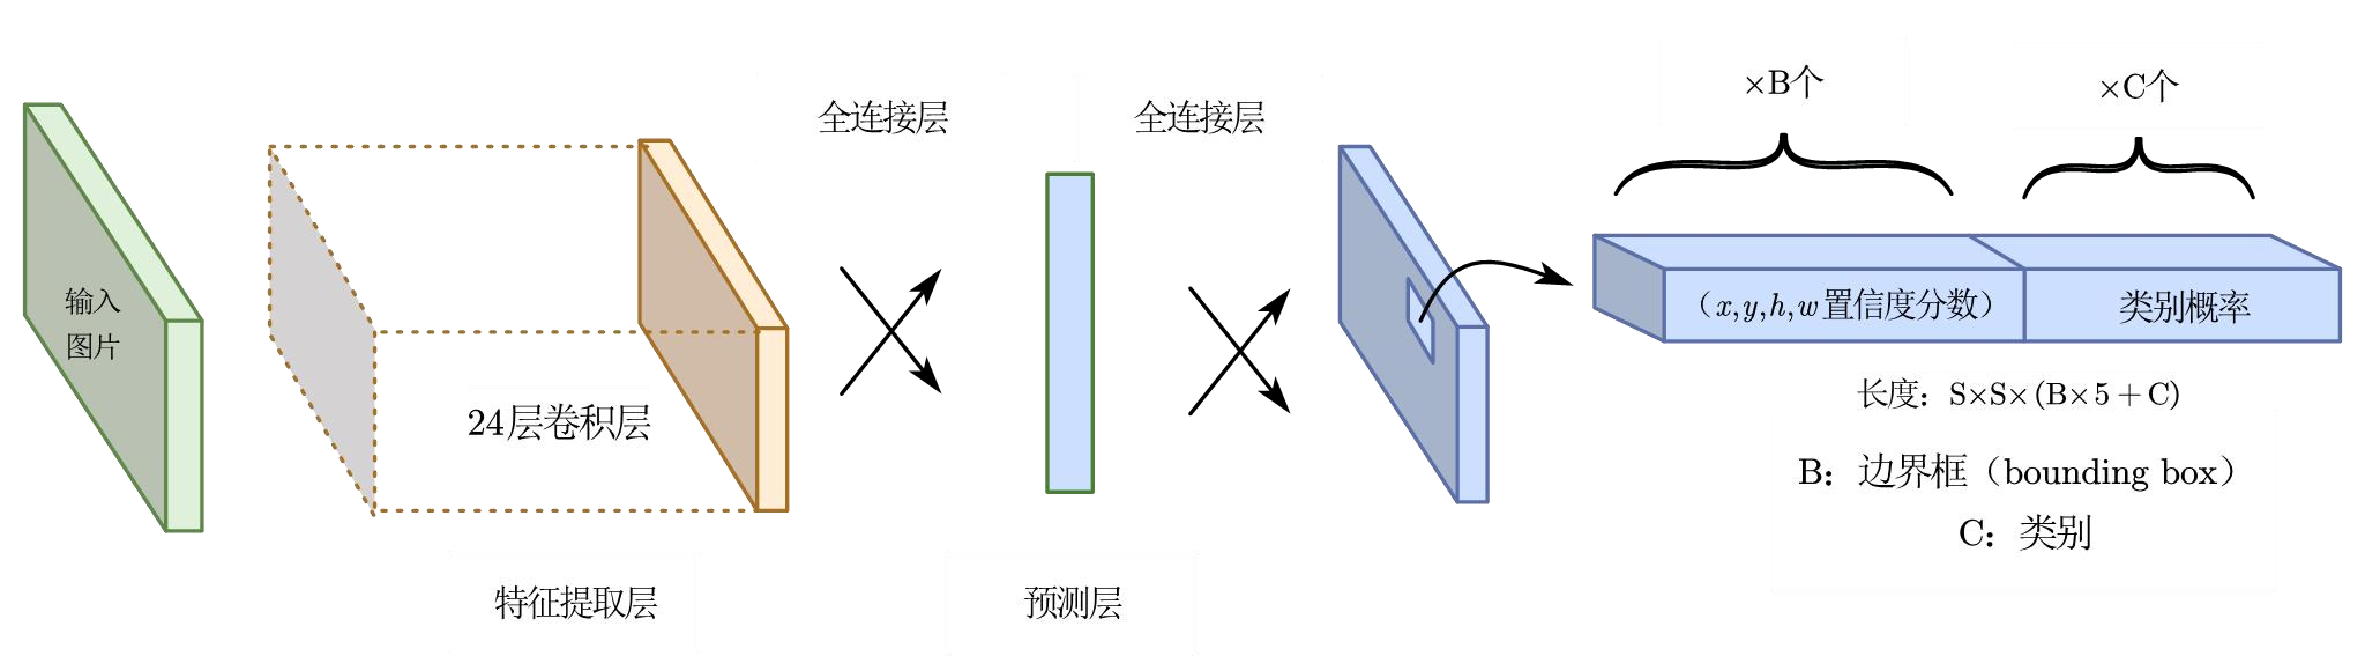
\includegraphics[width=0.8\textwidth]{figures/yolo神经网络结构.pdf}
    \caption{YOLO 的神经网络结构}
    \label{fig:yolo}
 \end{figure}

\subsubsection{YOLO 的损失函数}

基于均方误差(Sum of Squared Errors, SSE)的损失函数是机器学习中常用的损失函数,简单、容易优化 。同样 YOLO 网络中也是基于 SSE 构建来损失函数,如下:

\begin{equation}
loss = \sum_{i=0}^{S^2} coordError + iouError + classError
\end{equation}

由于以下两个原因,YOLO 团队对SSE进行了改进,以更好地平衡不同类型的误差:

\begin{enumerate}
  \item 在每个网格单元(grid cell)中,定位误差(localization error)、IOU 误差和分类误差(classification error)对总损失的影响存在显著差异,但 SSE 并未对这些误差进行区分处理。
  
  \item 图像中多数网格单元不包含目标物体,根据 YOLO 的设计,这些网格的 bounding box 的置信度(confidence)被设为 0。由于这些负样本数量庞大,其在梯度更新中的总贡献反而可能超过了包含目标的正样本,导致模型训练不稳定。
\end{enumerate}

为解决上述问题,YOLO 引入了一个改进的损失函数\textsuperscript{\cite{DZYX202210040}},在整体上实现了对定位误差、IOU 误差和分类误差的平衡。该损失函数的形式如下:

\begin{align}
\text{Loss Function} = & \lambda_{\text{coord}} \sum_{i=0}^{S^2} \sum_{j=0}^{B} \mathbf{1}_{ij}^{\text{obj}} \big[ (x_i - \hat{x}_i)^2 + (y_i - \hat{y}_i)^2 \big] \nonumber 
 + \lambda_{\text{coord}} \sum_{i=0}^{S^2} \sum_{j=0}^{B} \mathbf{1}_{ij}^{\text{obj}} \big[ (\sqrt{w_i} - \sqrt{\hat{w}_i})^2 \\
 &+ (\sqrt{h_i} - \sqrt{\hat{h}_i})^2 \big] \nonumber 
  + \sum_{i=0}^{S^2} \sum_{j=0}^{B} \mathbf{1}_{ij}^{\text{obj}} (C_i - \hat{C}_i)^2 \nonumber 
   + \lambda_{\text{noobj}} \sum_{i=0}^{S^2} \sum_{j=0}^{B} \mathbf{1}_{ij}^{\text{noobj}} (C_i - \hat{C}_i)^2 \nonumber \\
  &+ \sum_{i=0}^{S^2} \mathbf{1}_{i}^{\text{obj}} \sum_{C \in \text{classes}} (p_i(C) - \hat{p}_i(C))^2
\end{align}


式中 $x_i$ 和 $y_i$ 为预测目标的 $x$ 和 $y$ 轴坐标,$\hat{x}_i$ 和 $\hat{y}_i$ 为实际目标的 $x$ 和 $y$ 轴坐标;$w_i$ 和 $h_i$ 为预测目标的宽和高,$\hat{w}_i$ 和 $\hat{h}_i$ 为实际目标的宽和高;$C_i$ 为预测目标的类别,$\hat{C}_i$ 为实际目标的类别。第四项是对背景的置信度的预测。第五项是对物体类别的预测 $P_r(Class_i|Object)$,$p_i(C)$ 为预测目标的置信度,$\hat{p}_i(C)$ 为实际目标的置信度;$\lambda_{coord}$ 和$\lambda_{noobj}$是为了平衡各项 Loss 的比重所设定的权值,分别为 5 和 0.5。S 为每一个网格单元,B 为每一个边界框,obj为含有目标,noobj 为不含目标。

\begin{figure}[ht]
    \centering
    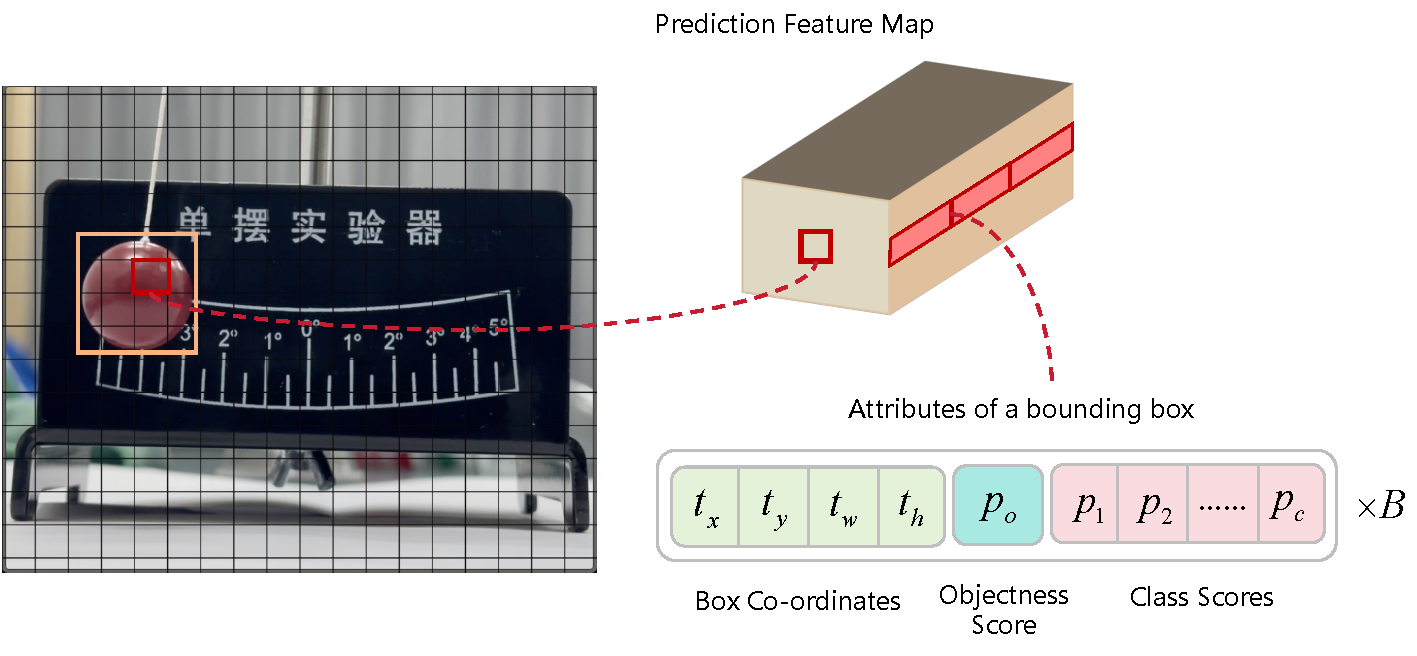
\includegraphics[width=0.9\textwidth]{figures/图片在网格中的处理.pdf}
    \caption{图片在网格中的处理过程}
    \label{fig:grid_process}
\end{figure}


\subsubsection{基于YOLO的摆球识别}
本文提出的基于深度学习 YOLO 的摆球识别方法能够定位视频中的摆球并返回其标。不同于基于区域预测的目标检测算法(Faster RCNN),YOLO 通过单个卷积神经网络检测整个图像回归目标的类别和位置,为了让卷积遍历整幅图像之后能够得到固定格式的预测大小,首先将图像调整为固定大小的尺寸640×640,再分成S×S 的非重叠的网格单元,然后每个单元负责检测出该单元可能拥有的 B 个边界框及其置信度,具体包含 5 个预测参数:x,y,w,h 和置信度。(x,y)代表目标的坐标,(w,h)代表目标外包矩形的宽度和高度,置信度用来通过阈值对预测结果进行取舍。 